\begin{figure*}[h]
	\centering{
    \begin{tabular}{ccc}
    	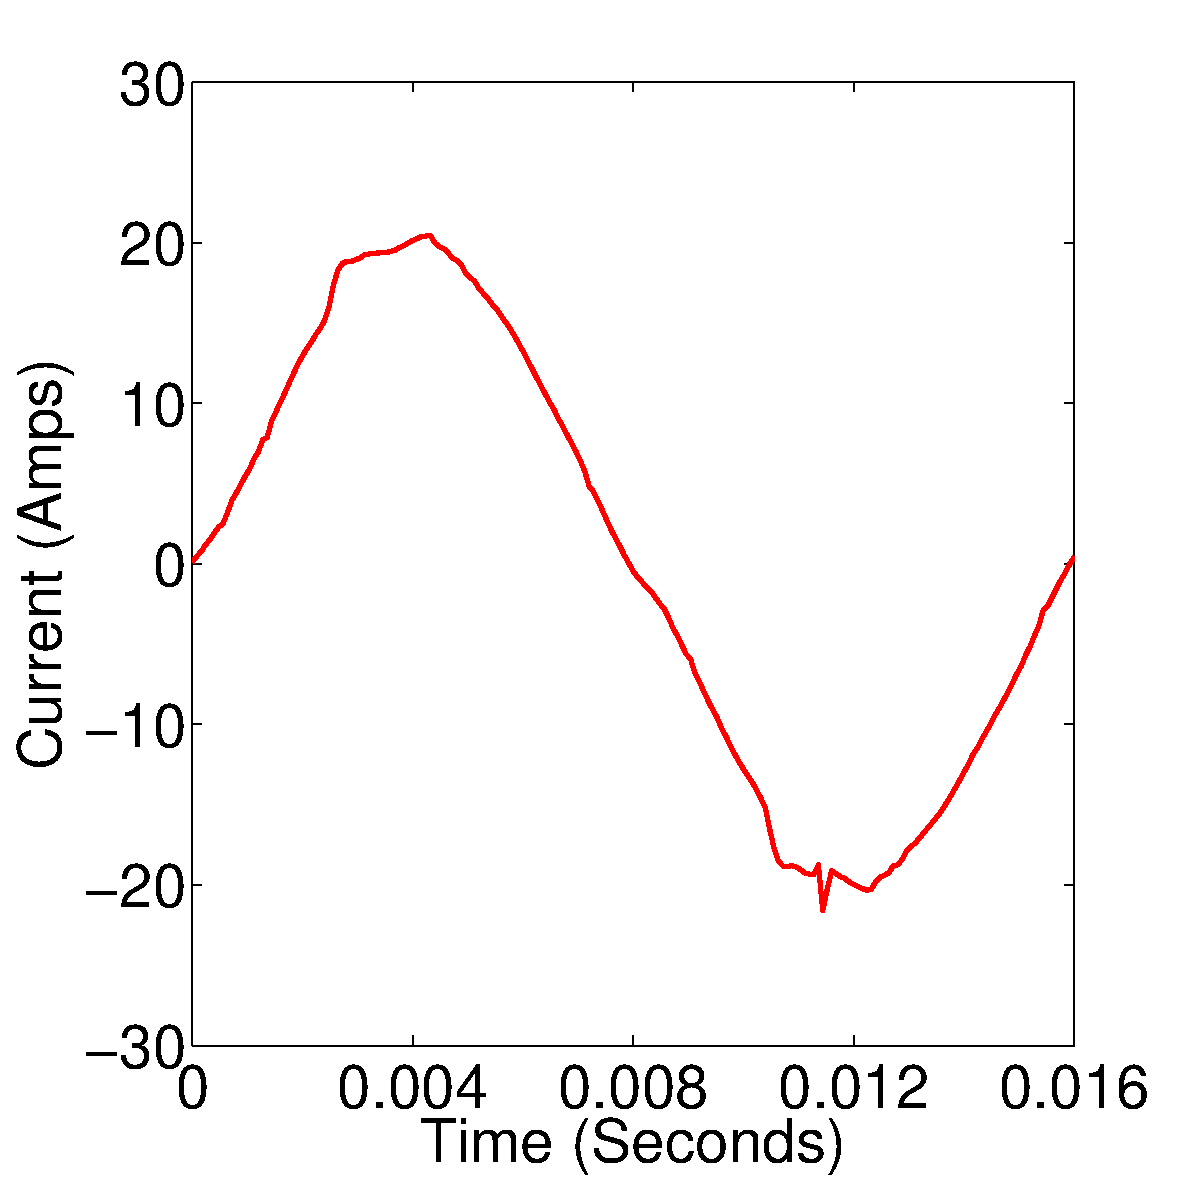
\includegraphics[width=0.3\textwidth]{figs/refrigeratorTransientSingle.pdf} \hspace{1em}&	
	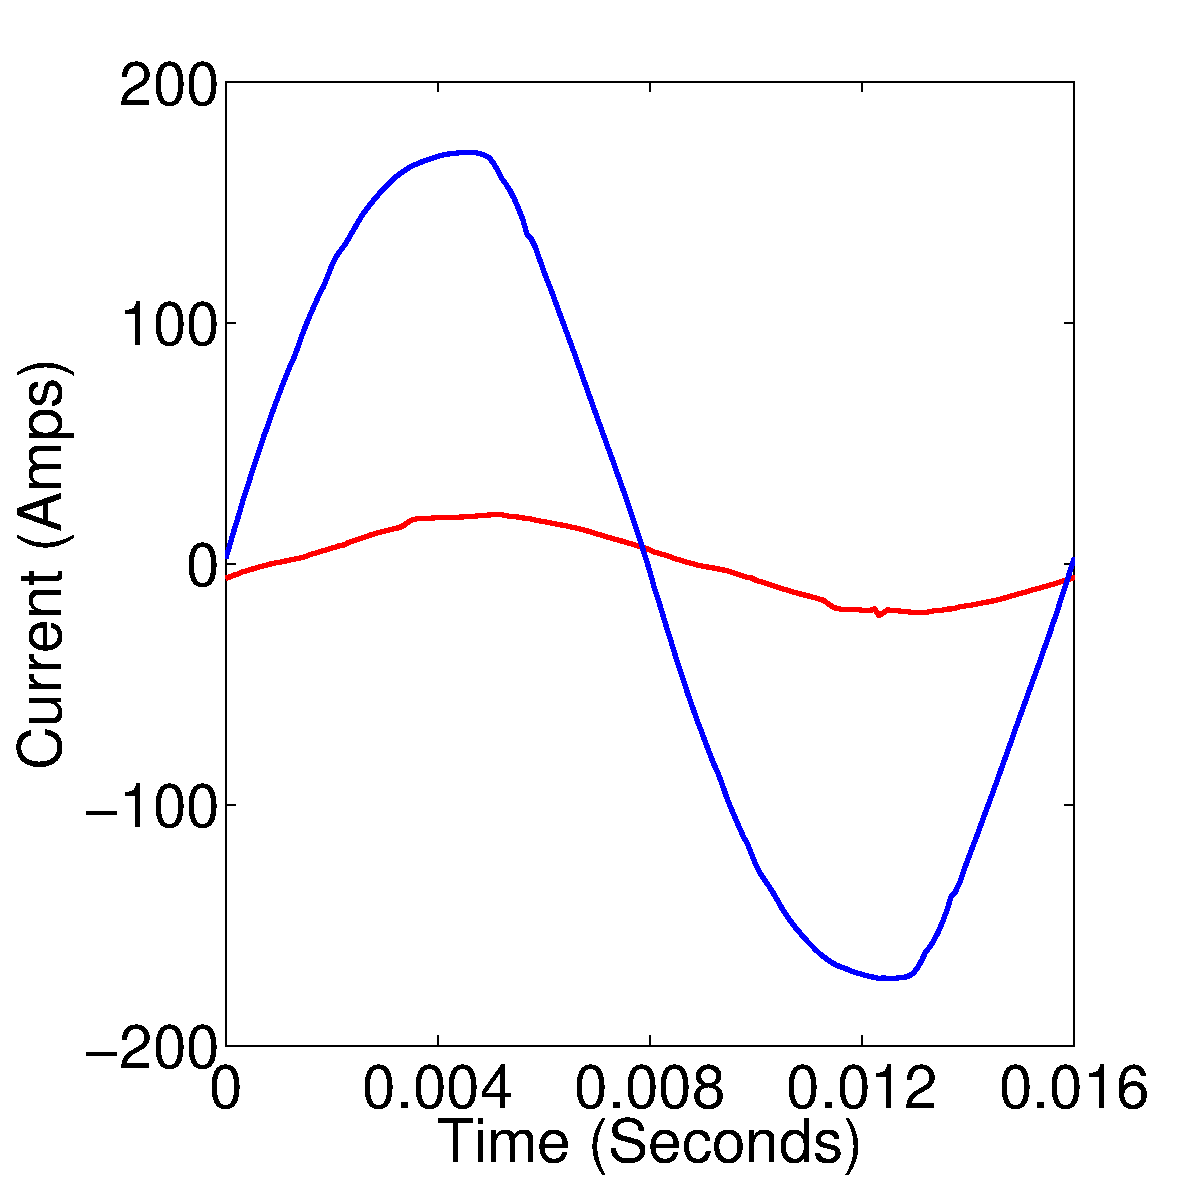
\includegraphics[width=0.3\textwidth]{figs/refrigeratorTransientCurrentVoltageSingle.pdf} \hspace{1em}&
	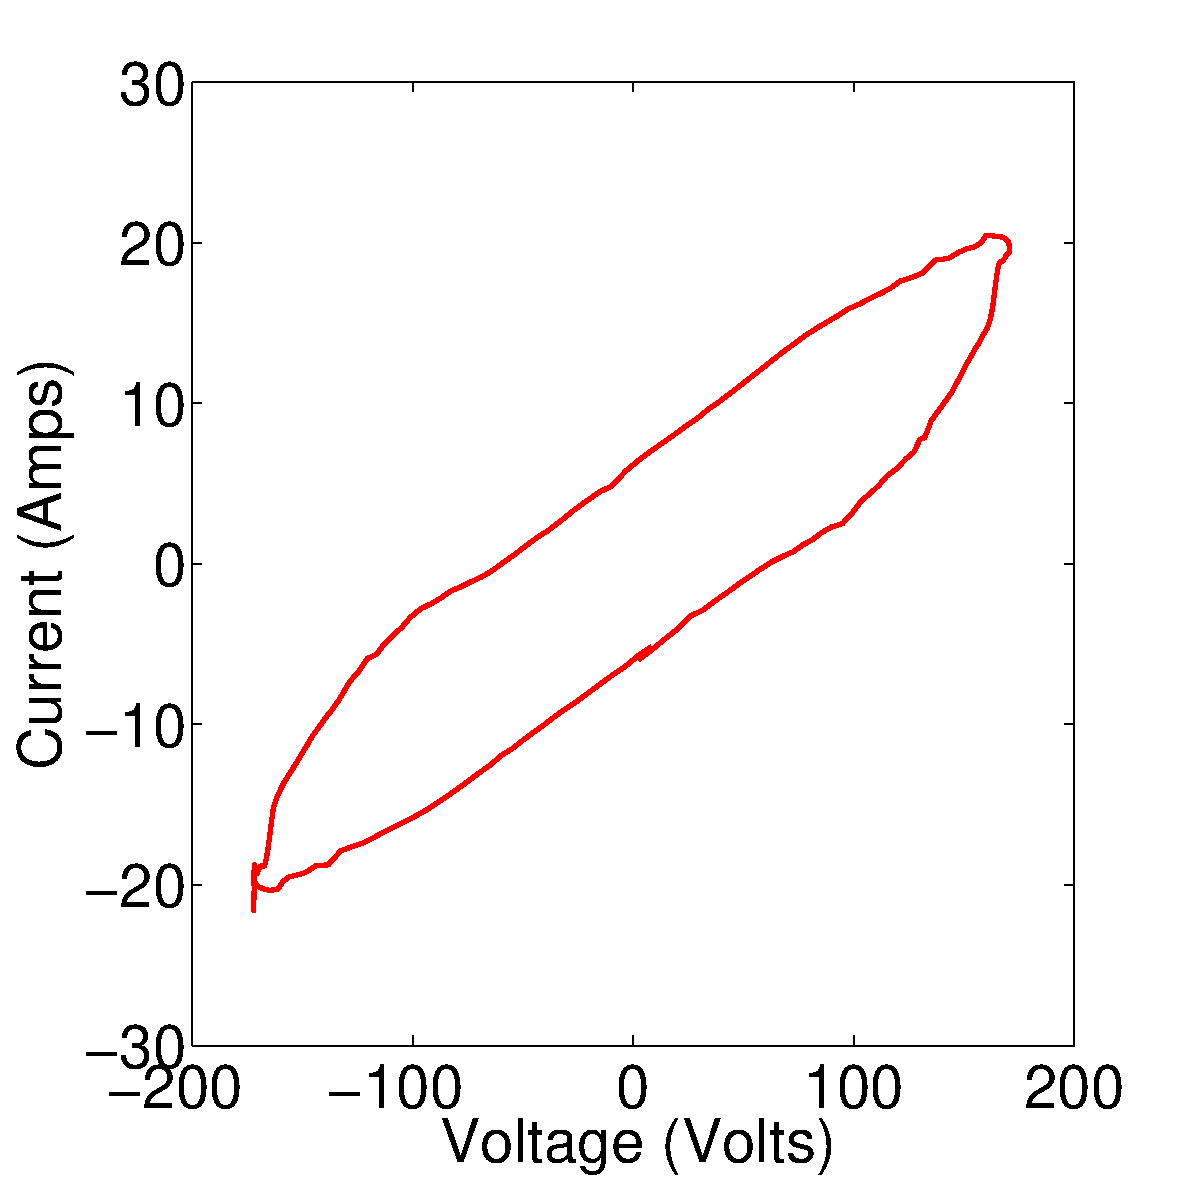
\includegraphics[width=0.3\textwidth]{figs/refrigeratorCurrentAgainstVoltageSingle.pdf} \tabularnewline

    (a) refrigerator & (c) refrigerator & (e) refrigerator \tabularnewline
        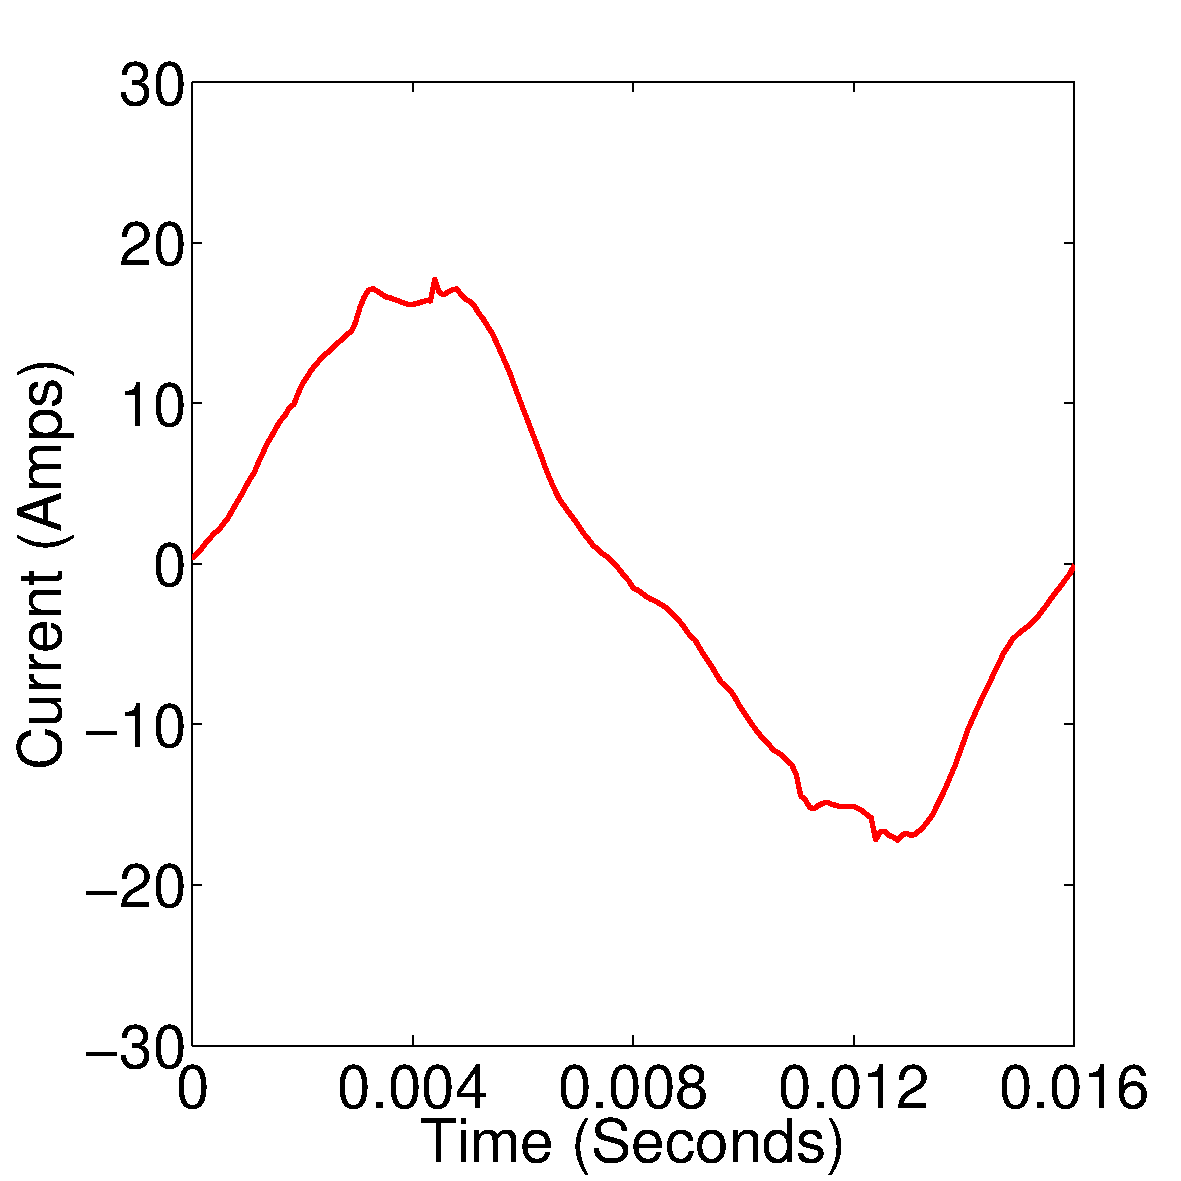
\includegraphics[width=0.3\textwidth]{figs/airCompressorTransientSingle.pdf} \hspace{1em}&	
        	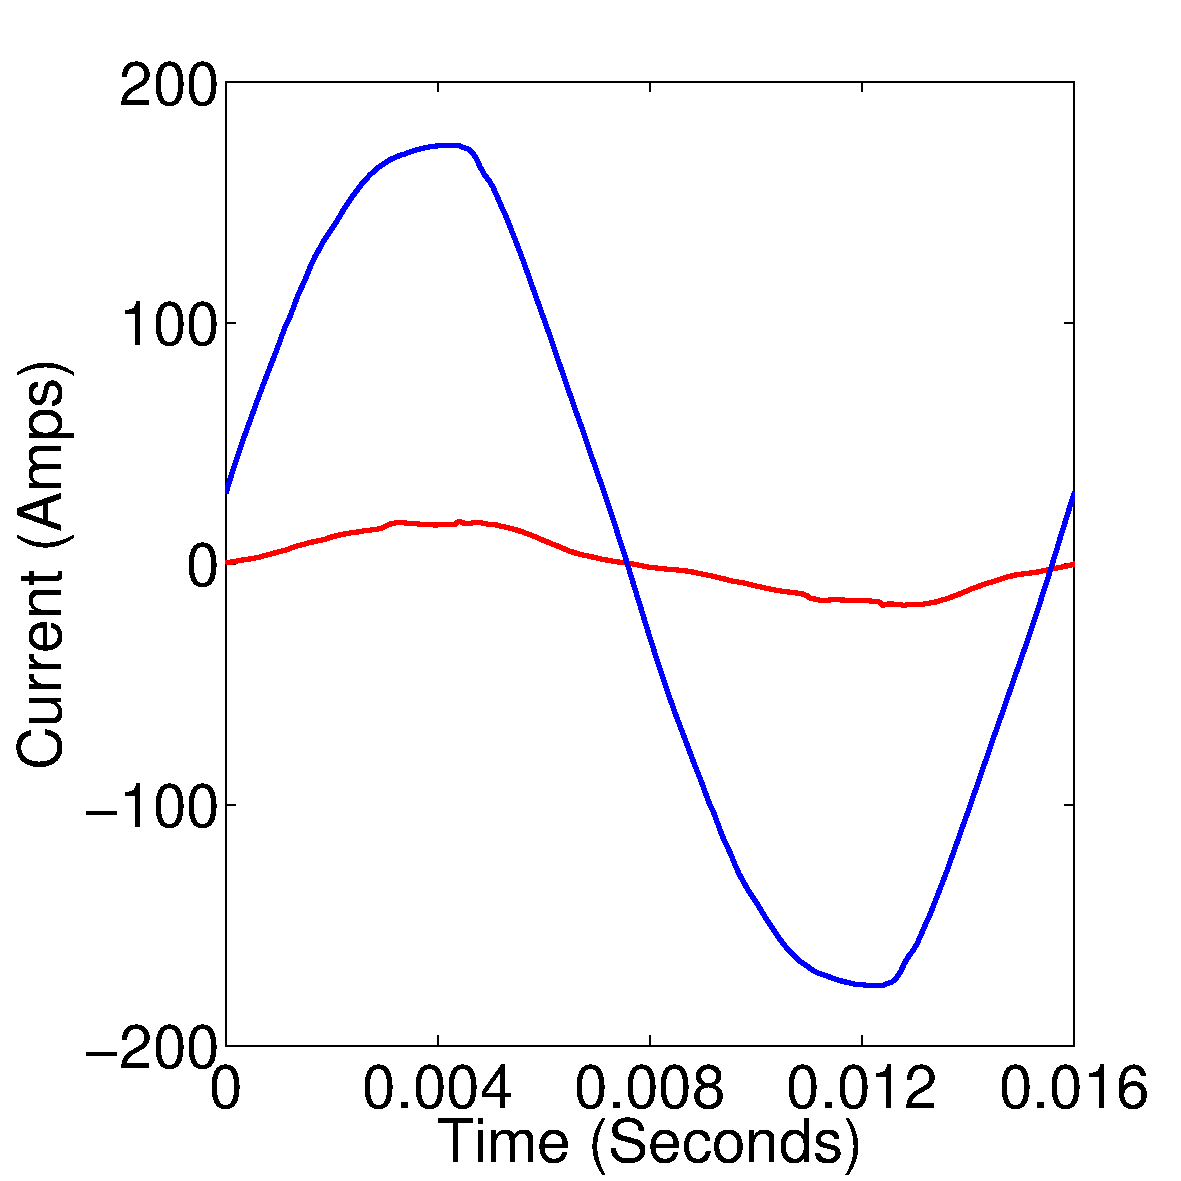
\includegraphics[width=0.3\textwidth]{figs/airCompressorTransientCurrentVoltageSingle.pdf}\hspace{1em}&	
	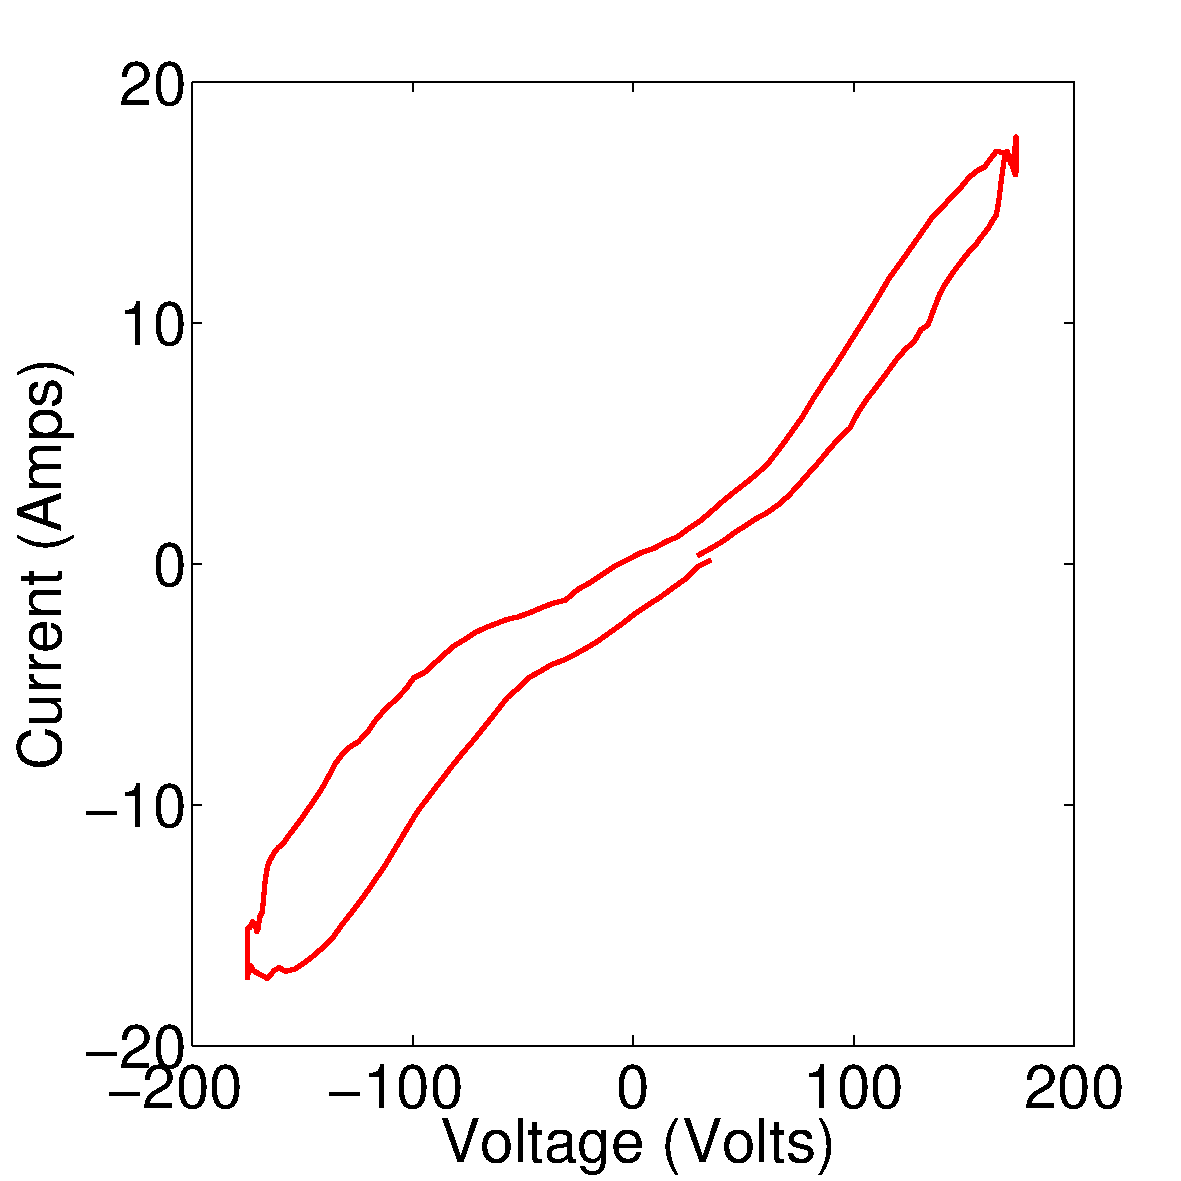
\includegraphics[width=0.3\textwidth]{figs/airCompressorCurrentAgainstVoltageSingle.pdf}\tabularnewline
    (b) air compressor & (d) air compressor & (f) air compressor \tabularnewline
    \end{tabular}
    }
	\caption{Current waveform of (a) a refrigerator and (b) an air compressor. The current and voltage of (c) a refrigerator and (c) an air compressor. The V-I trajectories of (e) a refrigerator and (f) an air compressor. }
	\label{fig_waveformTraj}
\end{figure*}